\documentclass[
    % handout,
    center,
    % aspectratio=169
]{beamer}

\usepackage[utf8]{inputenc}
\usepackage[english]{babel}
\usepackage{graphicx}
\usepackage{amsmath,amssymb,amsfonts}
\usepackage{array, booktabs, makecell}
\usepackage{tabularx}
\usepackage[ruled,vlined]{algorithm2e}

\graphicspath{../}

\title[Deep Learning Camera Pose Estimation]{\textsc{A Deep Learning Approach to\\Camera Pose Estimation}}
\author[Bozzo - Izzo]{Federico Izzo \and Francesco Bozzo}
\institute[UniTN]{University of Trento}
\date{January 12, 2022}

% \logo{\includegraphics[height=1.5cm]{logo.png}}
\usetheme{Madrid}
\definecolor{links}{HTML}{54489a}
\hypersetup{colorlinks,linkcolor=,urlcolor=links}
% \usetheme{metropolis} 


\begin{document}

\begin{frame}
    \titlepage
\end{frame}

% \AtBeginSection[]
% {
%     \begin{frame}{Table of Contents}
%         \begin{columns}[t]
%             \column{.45\textwidth}
%             \tableofcontents[sections=1-2, currentsection]

%             \column{.45\textwidth}
%             \tableofcontents[sections=3-5, currentsection]
%         \end{columns}
%     \end{frame}
% }

\section{Introduction}
\begin{frame}{Introduction}
    With this work we are going to present:
    \begin{itemize}
        \item the camera pose estimation problem;
        \item the exploration of labeled dataset generation techniques applied on Povo 1 second floor;
        \item relative and absolute pose estimation deep learning models;
        \item the post-processing of the model outputs;
        \item the model deployment using a FastAPI web-server.
    \end{itemize}
\end{frame}

% what is camera pose estimation: introdution image (with formulas?)
\begin{frame}{Camera Pose Estimation}
    \begin{columns}
        \column{0.45\textwidth}
        The \textbf{camera pose estimation} problem aims to find the function $E$ that, given an \textbf{image} $I_c$, returns the \textbf{position} $x_c$ and \textbf{orientation} $q_c$ of the camera.
        \[
            E(I_c) = (x_c, q_c)
        \]

        \column{0.50\textwidth}
        \begin{figure}
            \centering
            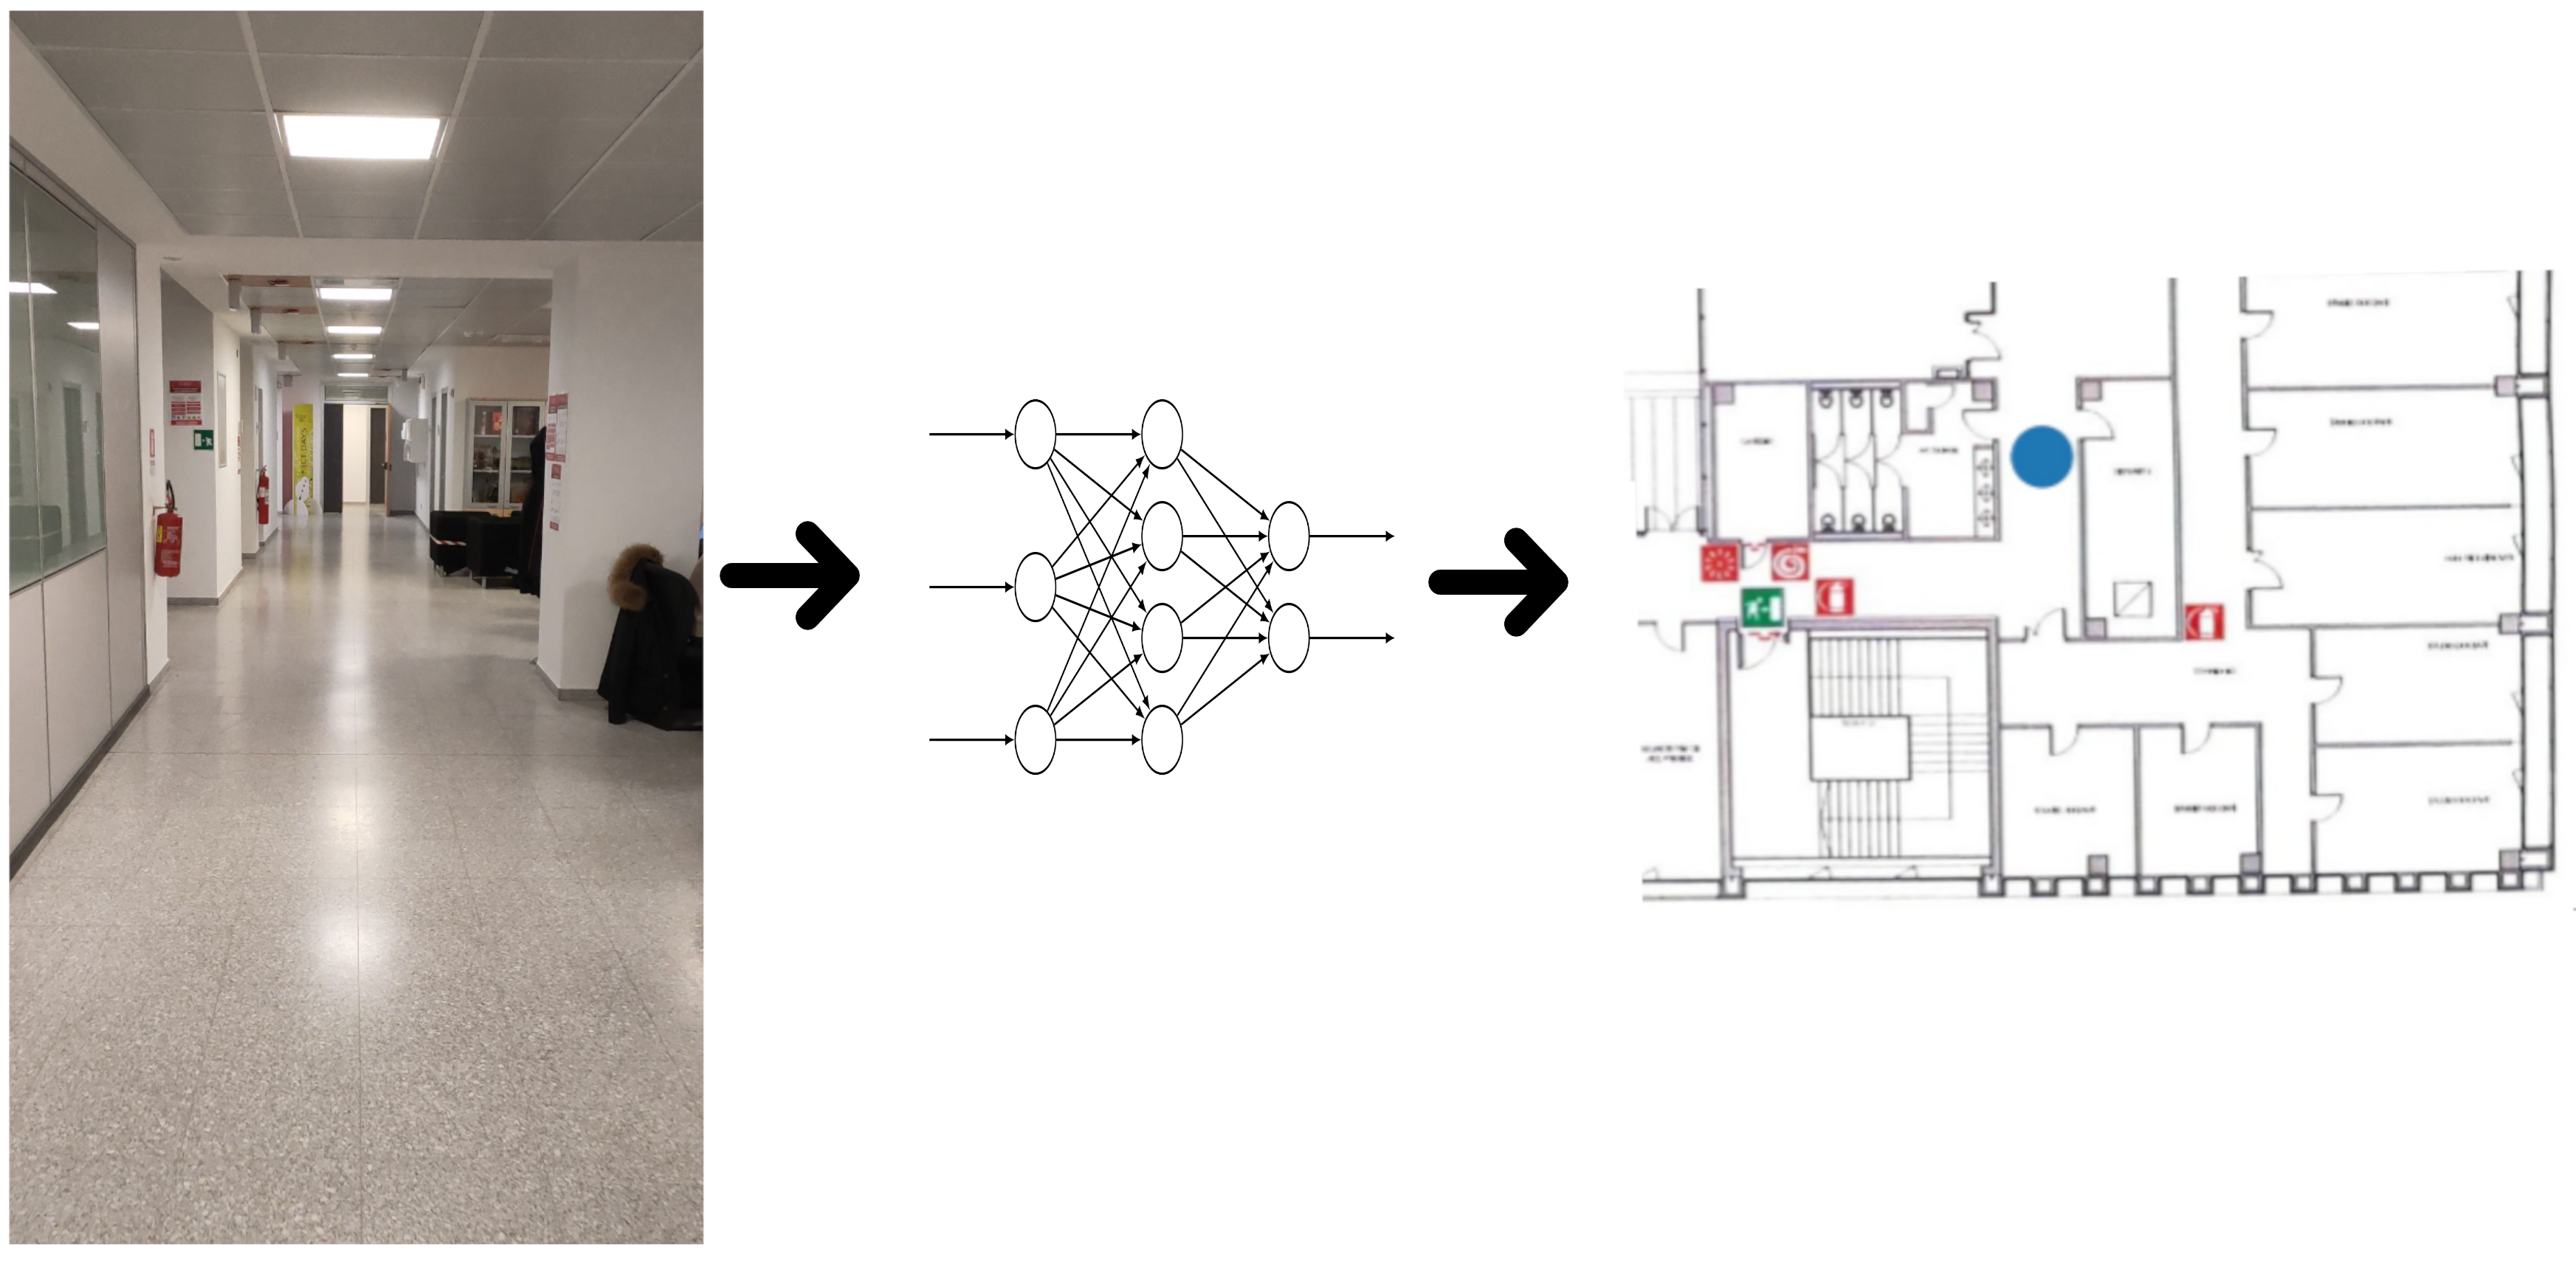
\includegraphics[width=0.9\textwidth]{../imgs/introduction_example.png}
            \caption{Example of camera relocalization.}
        \end{figure}
    \end{columns}
\end{frame}

\section{Dataset}
% presentation of the 4 different attempts for dataset generation
\begin{frame}{Different Approaches for Dataset Generation}
    We have considered four different techniques:
    \begin{itemize}
        \item \textbf{IMU sensors}: not enough accurate;
        \item \textbf{digital video}: not available in the university environment;
        \item \textbf{motion capture system}: difficult to associate with a recorder video;
        \item \textbf{structure from motion}: our choice (COLMAP).
    \end{itemize}
\end{frame}
% COLMAP: introduction with some examples
\begin{frame}{COLMAP - Structure From Motion}
    COLMAP is \textbf{structure from motion} tool that allows to reconstruct a 3D representation of an environment using images of it. During the process, it also computes camera poses in an arbitrary reference system.
    \vspace{10px}
    \begin{figure}
        \centering
        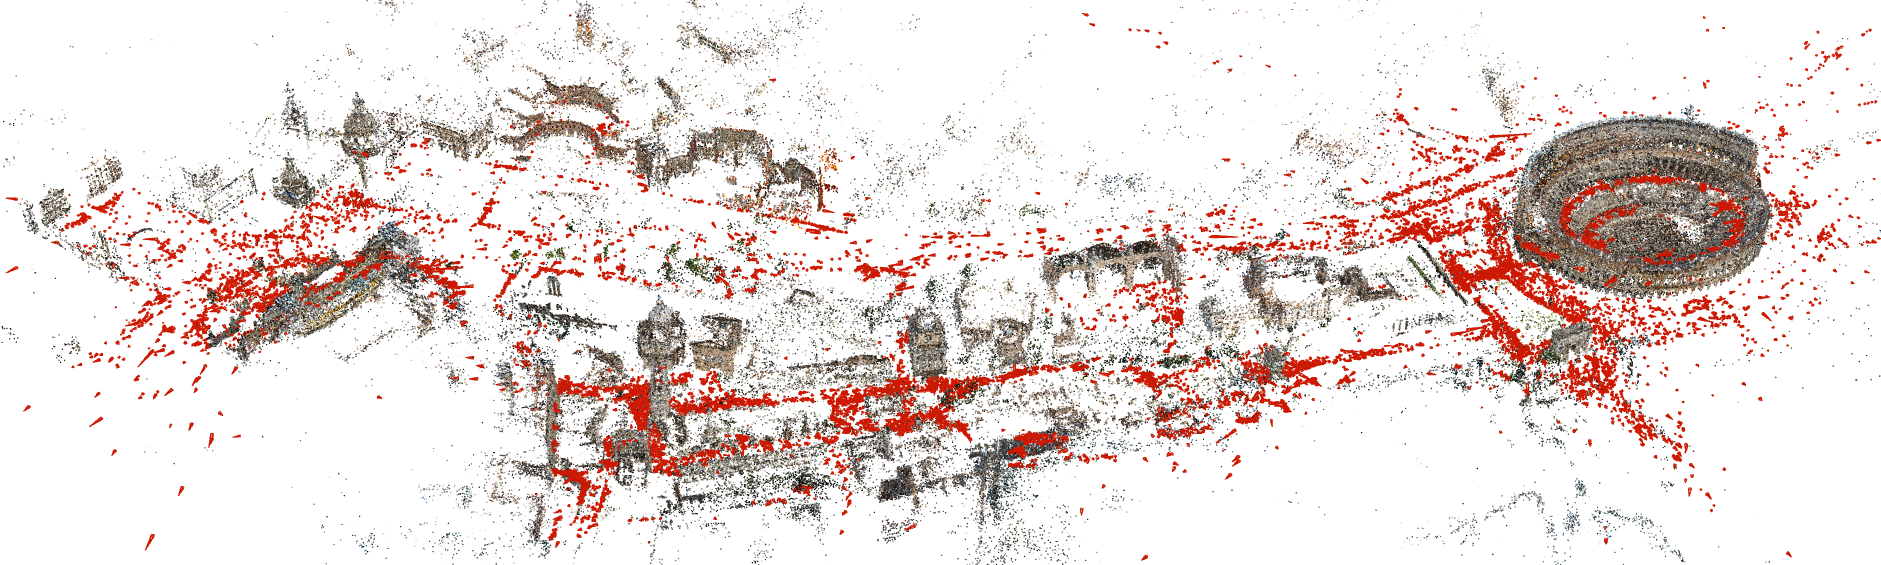
\includegraphics[width=0.8\textwidth]{../imgs/colmap_rome.png}
        \caption{COLMAP reconstruction of central Rome using 21K photos.}
    \end{figure}
\end{frame}
% Uni Povo2: some screens and stats
\begin{frame}{Povo 1 Second Floor Dataset}
    \begin{columns}
        \column{0.45\textwidth}
        \begin{figure}
            \centering
            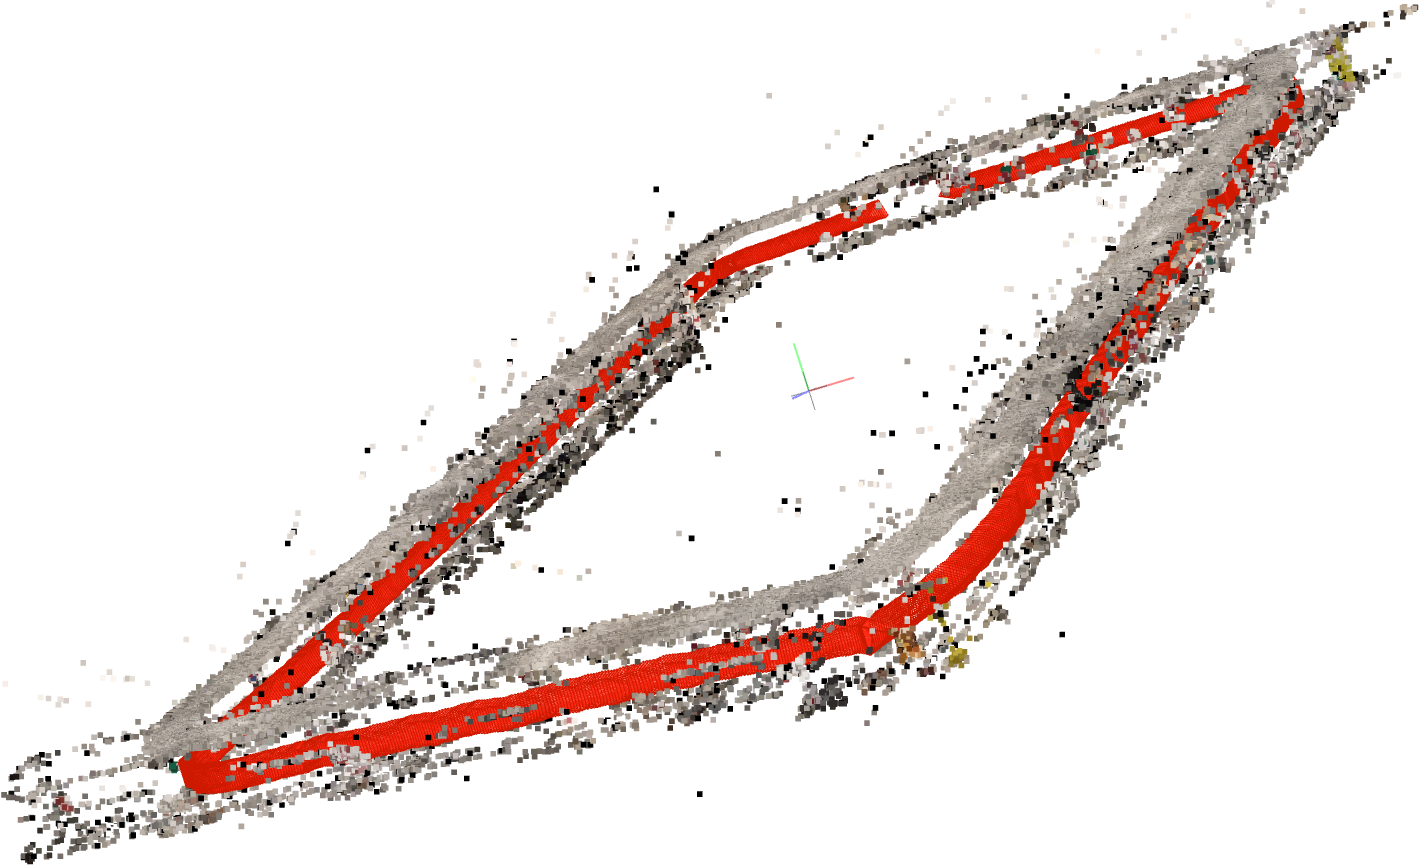
\includegraphics[width=0.9\textwidth]{../imgs/extracted_features_colmap.png}
            \caption{COLMAP reconstruction of Povo 1 second floor.}
        \end{figure}

        \column{0.45\textwidth}
        After many failed attempts, we managed to create a COLMAP reconstruction of \textbf{Povo 1 second floor}. The red line represents the camera trajectory and other points are the extracted features.
    \end{columns}
\end{frame}

% CRS alignment
\begin{frame}{Coordinate Reference System Alignment}
    \begin{columns}
        \column{0.50\textwidth}
        Some steps are required to align COLMAP's arbitrary \textbf{coordinate reference system (CRS)} with respect to the real world:
        \begin{enumerate}
            \item \textbf{scale}: align unit of measures;
            \item \textbf{translate}: align origins;
            \item \textbf{rotate}: align axes.
        \end{enumerate}

        \column{0.45\textwidth}
        \begin{figure}
            \centering
            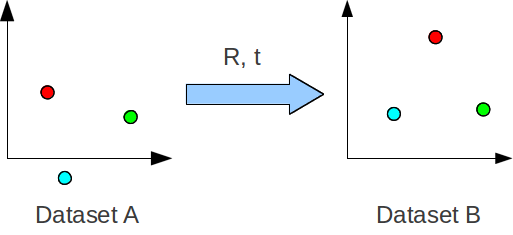
\includegraphics[width=0.9\textwidth]{../imgs/rigid_trasform.png}
            \caption{Rigid transformation.}
        \end{figure}
    \end{columns}
\end{frame}

\section{Models}
\subsection{MeNet}
\begin{frame}{The MeNet Model for Relative Pose Estimation}
    \begin{columns}
        \column{0.45\textwidth}
        \begin{figure}
            \centering
            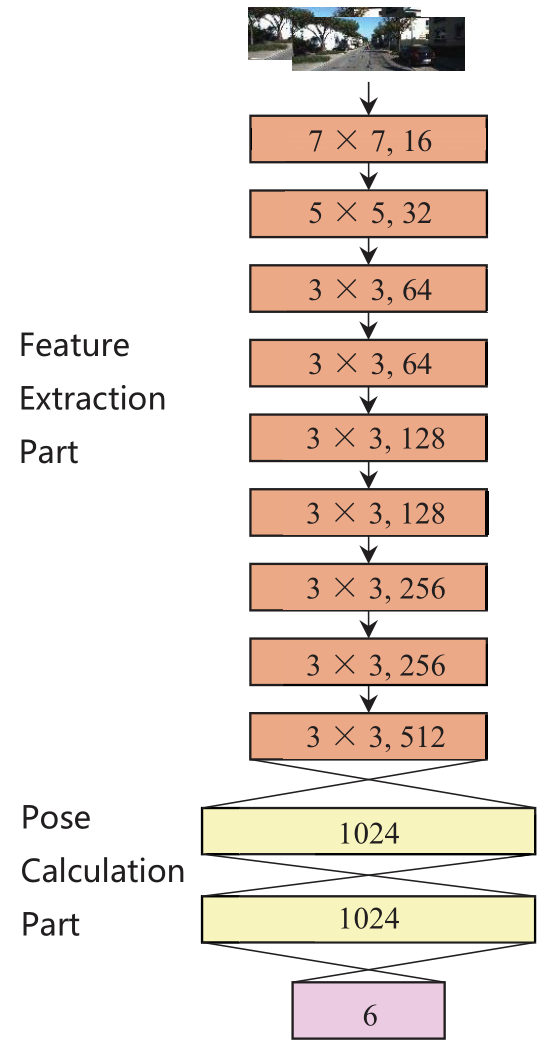
\includegraphics[width=0.9\textwidth]{../imgs/menet_structure.png}
            \caption{MeNet model architecture.}
        \end{figure}

        \column{0.45\textwidth}
        The \textbf{MeNet} model is targeted for \textbf{relative pose estimation}.
        The input of the network consists in a stack of two images: the goal is to estimate the relative pose of the second image with respect to the first one.
    \end{columns}
\end{frame}
\subsection{PoseNet}
\begin{frame}{The PoseNet Model for Absolute Pose Estimation}
    \begin{columns}
        \column{0.45\textwidth}
        \begin{figure}
            \centering
            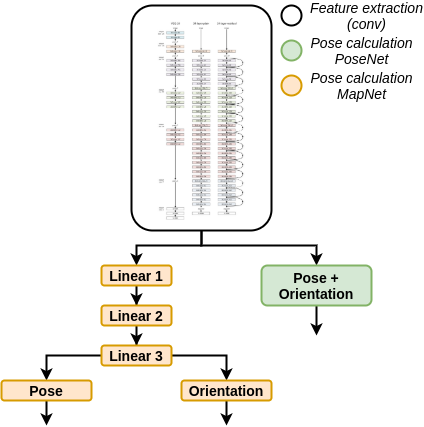
\includegraphics[width=0.9\textwidth]{../imgs/mapnet_posenet_structure.png}
            \caption{PoseNet model architecture.}
        \end{figure}

        \column{0.45\textwidth}
        The \textbf{PoseNet} model for absolute pose estimation is made up by two components:
        \begin{itemize}
            \item feature extraction through a sequence of convolutional layers (\emph{backend});
            \item pose regression on the extracted features using linear layers.
        \end{itemize}
    \end{columns}
\end{frame}
% PoseNet loss. General loss with h function (see MapNet loss in the report) with loss table and plot
\begin{frame}{The PoseNet Loss Function}
    \begin{columns}
        \column{0.45\textwidth}
        \begin{figure}
            \centering
            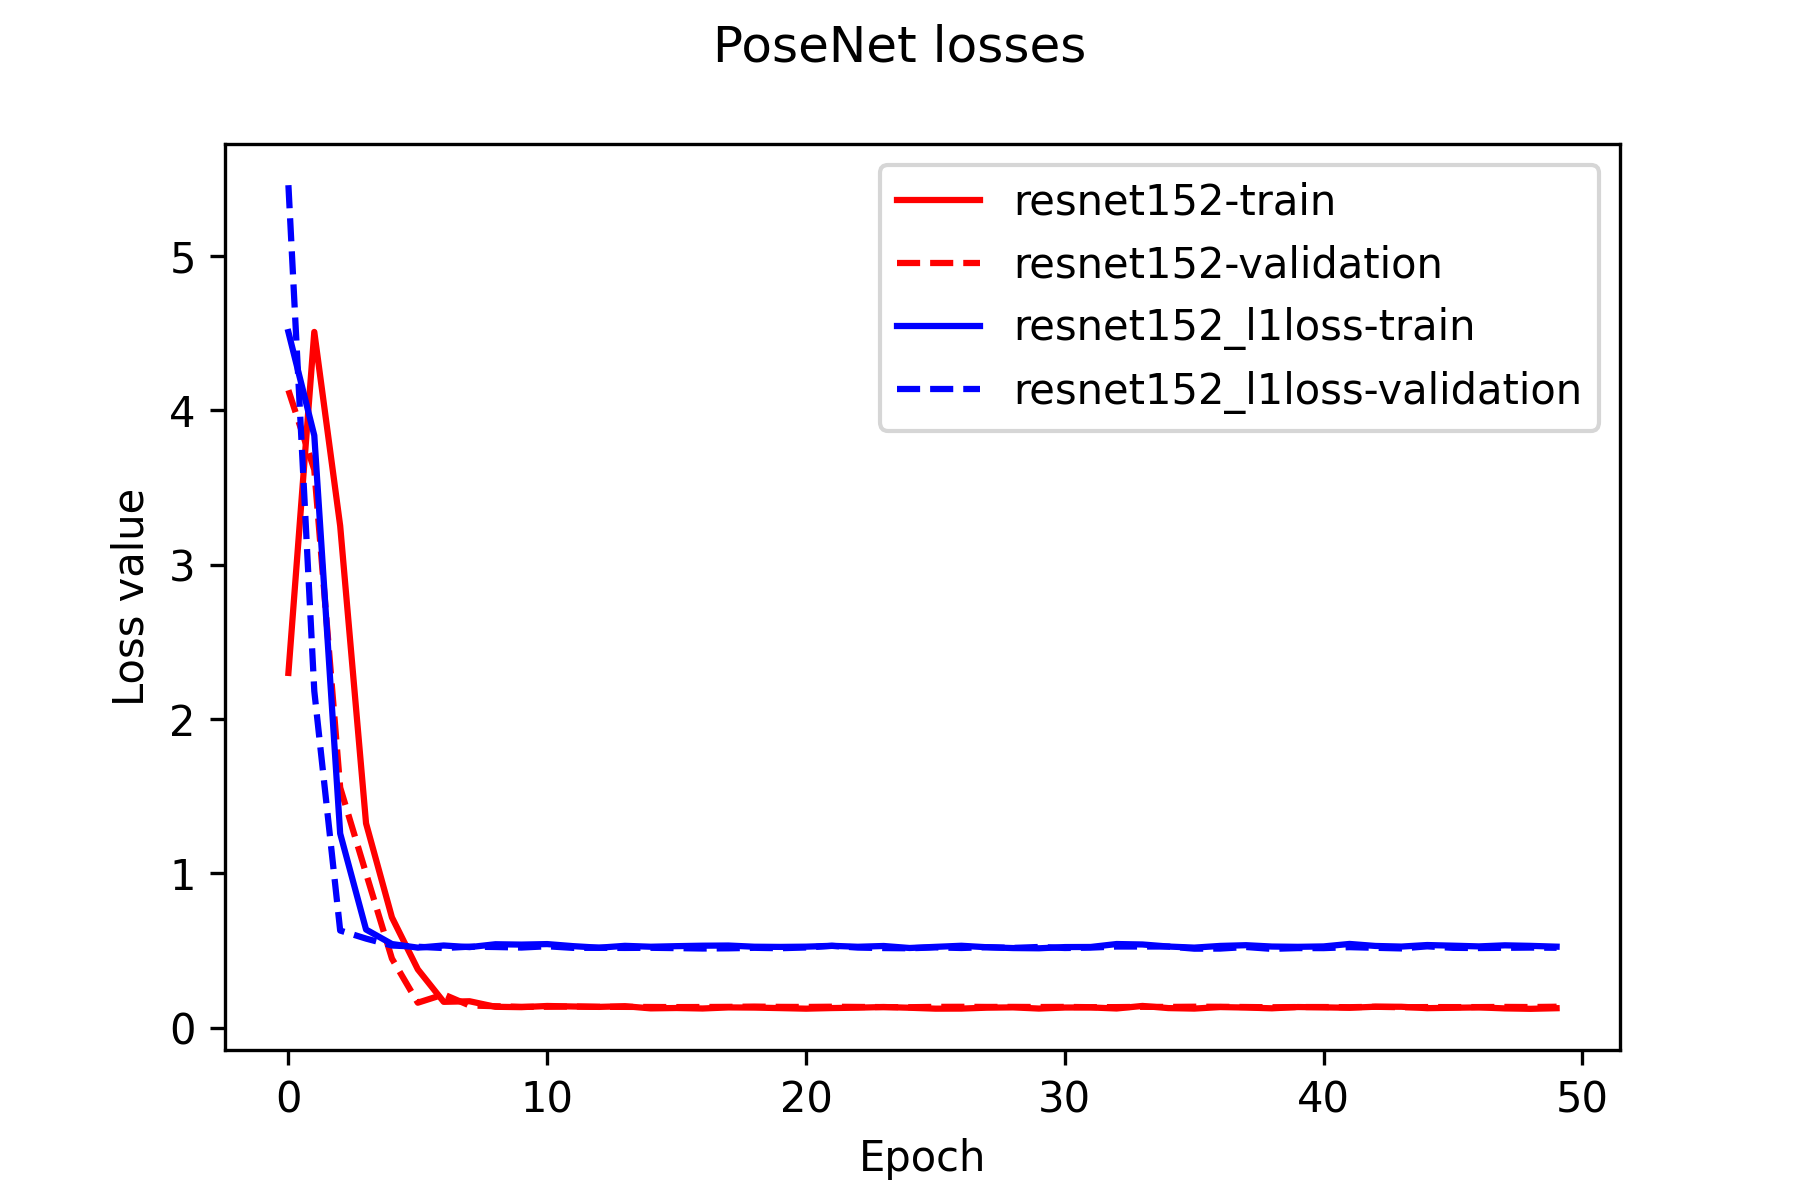
\includegraphics[width=0.9\textwidth]{../imgs/posenet_losses.png}
            \caption{PoseNet losses trend during training.}
        \end{figure}

        \column{0.45\textwidth}
        \begin{table}[htbp]
            \begin{center}
                \footnotesize
                \begin{tabular}{lrr}
                    \toprule
                    Loss            & \thead{Position                  \\Error} & \thead{Rotation\\Error} \\
                    \midrule
                    SmoothedL1Loss  & \textbf{0.594}  & \textbf{0.139} \\
                    L1Loss          & 0.906           & 0.226          \\
                    MSE             & NaN             & NaN            \\
                    $\alpha \neq 1$ & NaN             & NaN            \\
                    \bottomrule
                \end{tabular}
                \caption{PoseNet losses comparison.}
                \label{tab:posenet-losses}
            \end{center}
        \end{table}
        \begin{multline*}
            Loss(w) = \frac{1}{N} \sum\limits_{i=1}^N h(P^i, \hat{P}^i) \\
            + \alpha h(Q^i, \hat{Q}^i)
        \end{multline*}
    \end{columns}
\end{frame}
% PoseNet trajectory with 2000cm error
\begin{frame}{PoseNet Results}
    \begin{figure}
        \centering
        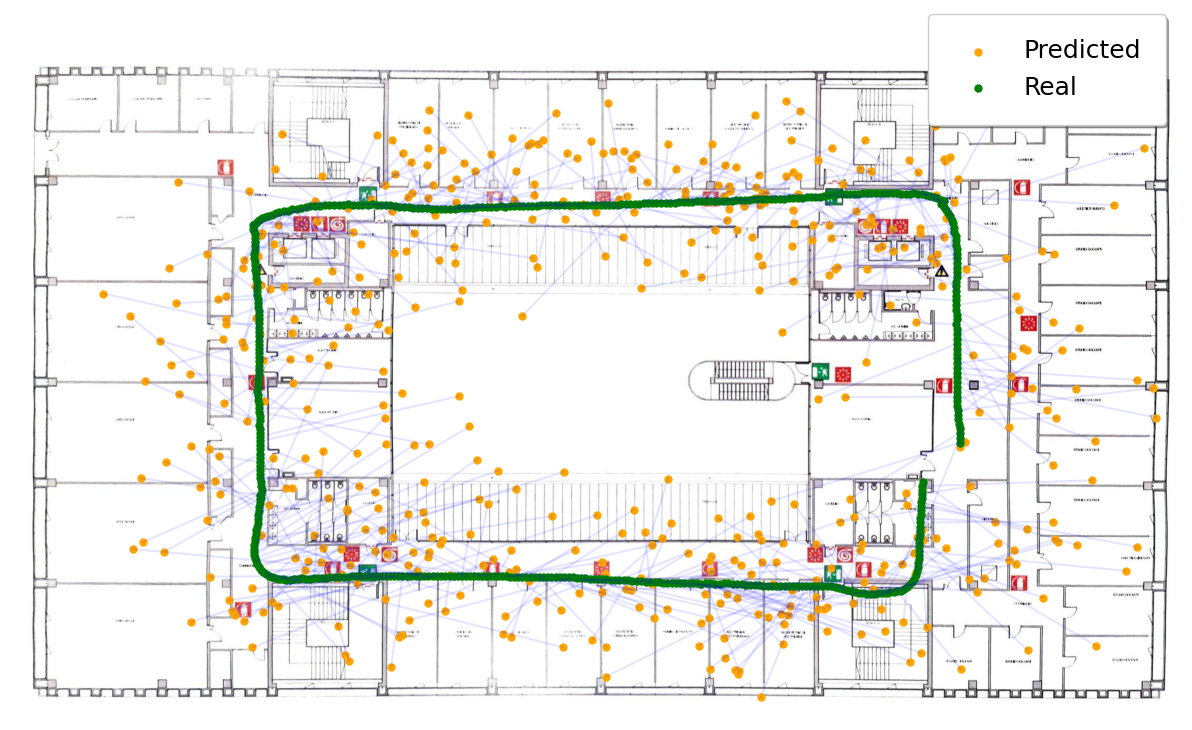
\includegraphics[width=0.9\textwidth]{../imgs/posenet_map.png}
        \caption{PoseNet predictions for our custom dataset. Error = $\sim 2000cm$.}
    \end{figure}
\end{frame}

% Absolute pose estimation models with transfer learning + backend table on ImageNet
\subsection{MapNet}
\begin{frame}{The MapNet Model for Absolute Pose Estimation}
    \begin{columns}
        \column{0.45\textwidth}
        \begin{figure}
            \centering
            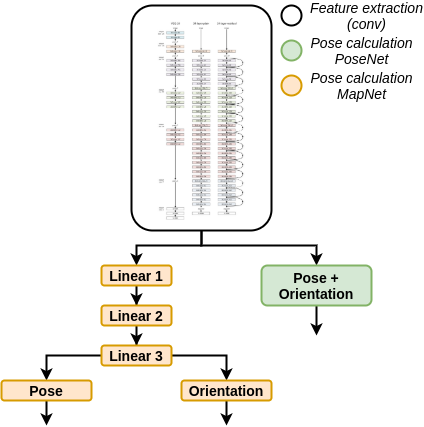
\includegraphics[width=0.9\textwidth]{../imgs/mapnet_posenet_structure.png}
            \caption{MapNet model architecture.}
        \end{figure}

        \column{0.45\textwidth}
        The \textbf{MapNet} model for absolute pose estimation represents an evolution of the PoseNet model with improvements:
        \begin{itemize}
            \item increase the number of final linear layers;
            \item penalize both absolute and relative errors in the loss.
        \end{itemize}
    \end{columns}
\end{frame}
% MapNet loss. General loss with h function with loss table and plot
\begin{frame}{The MapNet Loss Function}
    \begin{columns}
        \column{0.45\textwidth}
        \begin{figure}
            \centering
            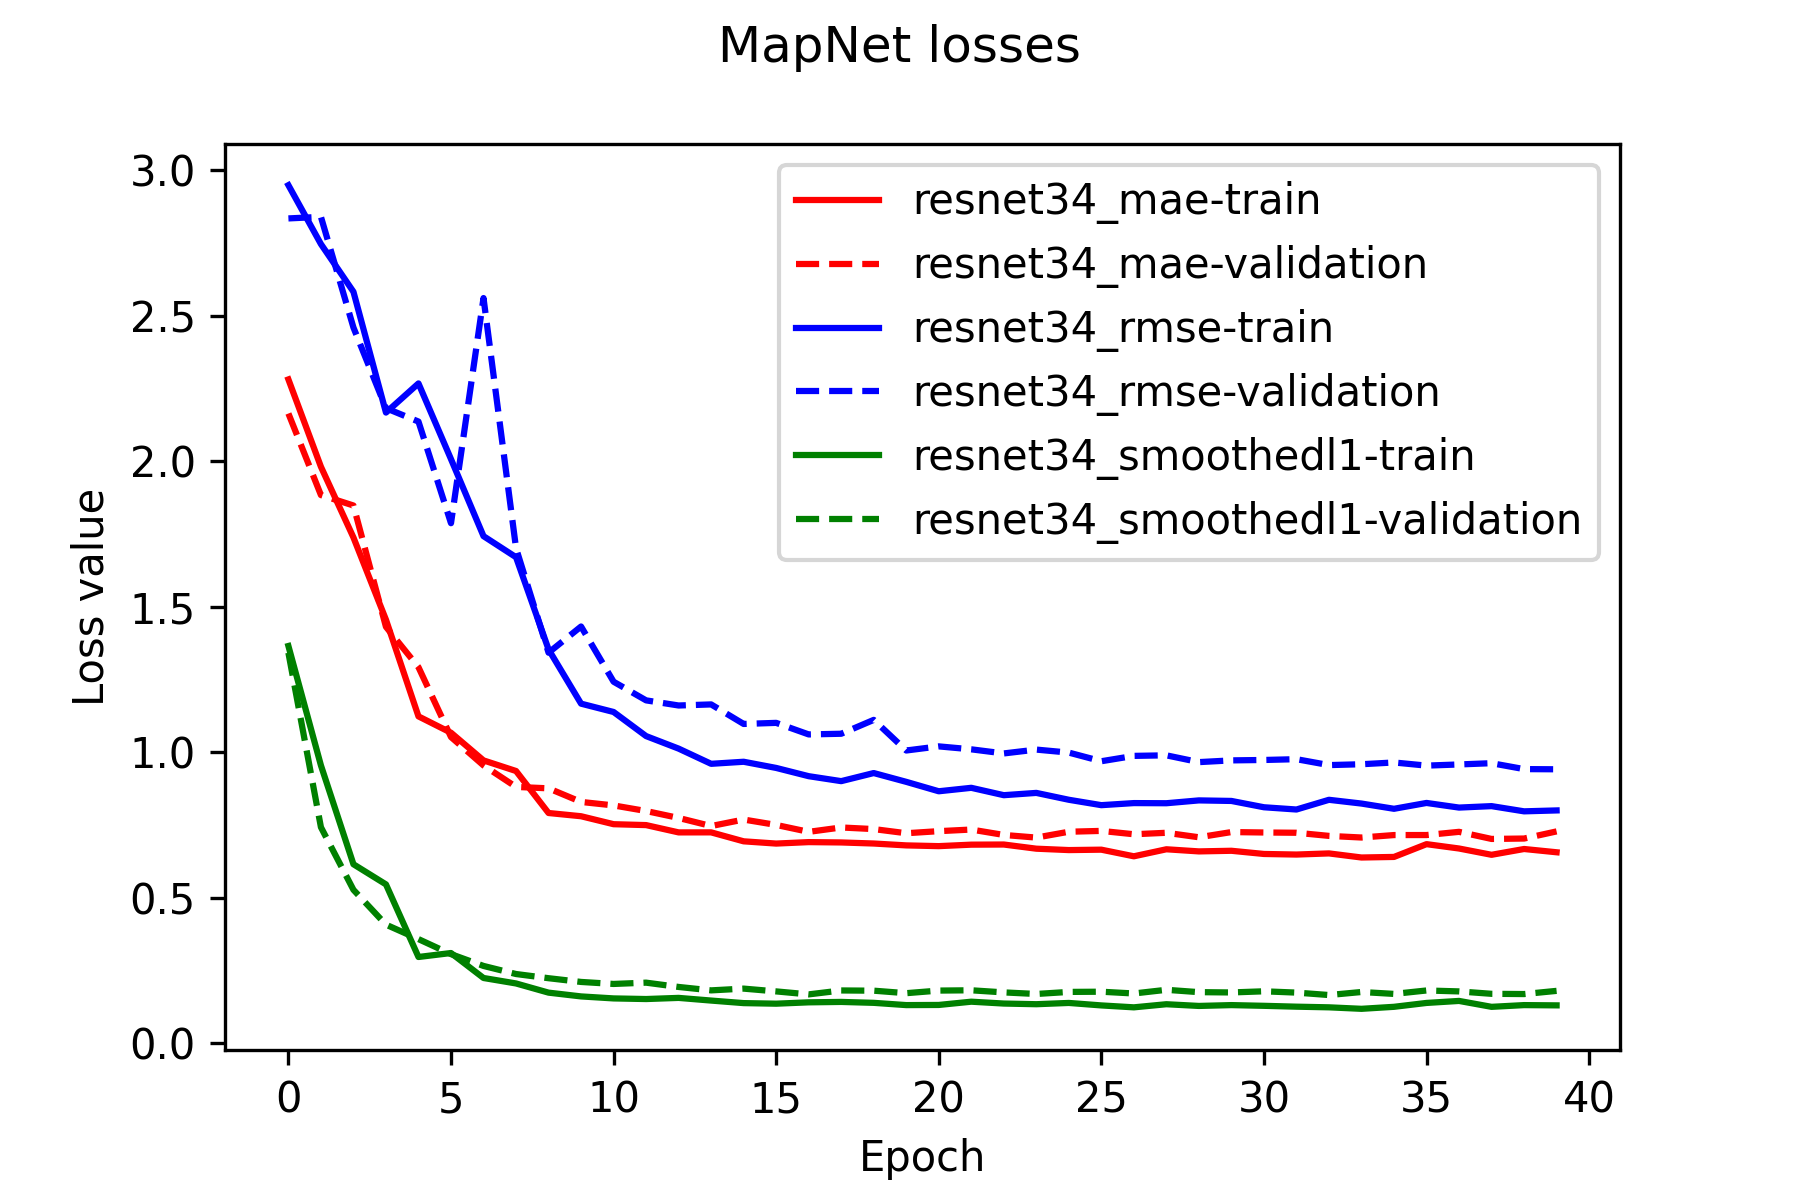
\includegraphics[width=0.9\textwidth]{../imgs/mapnet_losses.png}
            \caption{MapNet losses trend during training.}
        \end{figure}

        \column{0.45\textwidth}
        \begin{table}[htbp]
            \begin{center}
                \footnotesize
                \begin{tabular}{lrr}
                    \toprule
                    Loss           & \thead{Position                  \\Error} & \thead{Rotation\\Error} \\
                    \midrule
                    L1Loss         & 0.227           & 0.042          \\
                    SmoothedL1Loss & 0.187           & 0.076          \\
                    RMSE           & \textbf{0.187}  & \textbf{0.038} \\
                    \bottomrule
                \end{tabular}
                \caption{MapNet losses comparison.}
                \label{tab:mapnet-losses}
            \end{center}
        \end{table}
        \begin{multline*}
            L_\mathcal{D}(\Theta) = \sum\limits_{i=1}^{|\mathcal{D}|} h([\hat{P}^i \hat{Q}^i], [P^i Q^i]) \\
            + \alpha\sum\limits_{i,j=1, i\neq j}^{|\mathcal{D}|} h([\hat{P}^{ij} \hat{Q}^{ij}], [P^{ij} Q^{ij}])
        \end{multline*}
    \end{columns}
\end{frame}
% MapNet trajectory with 153cm error
\begin{frame}{MapNet Results}
    \begin{figure}
        \centering
        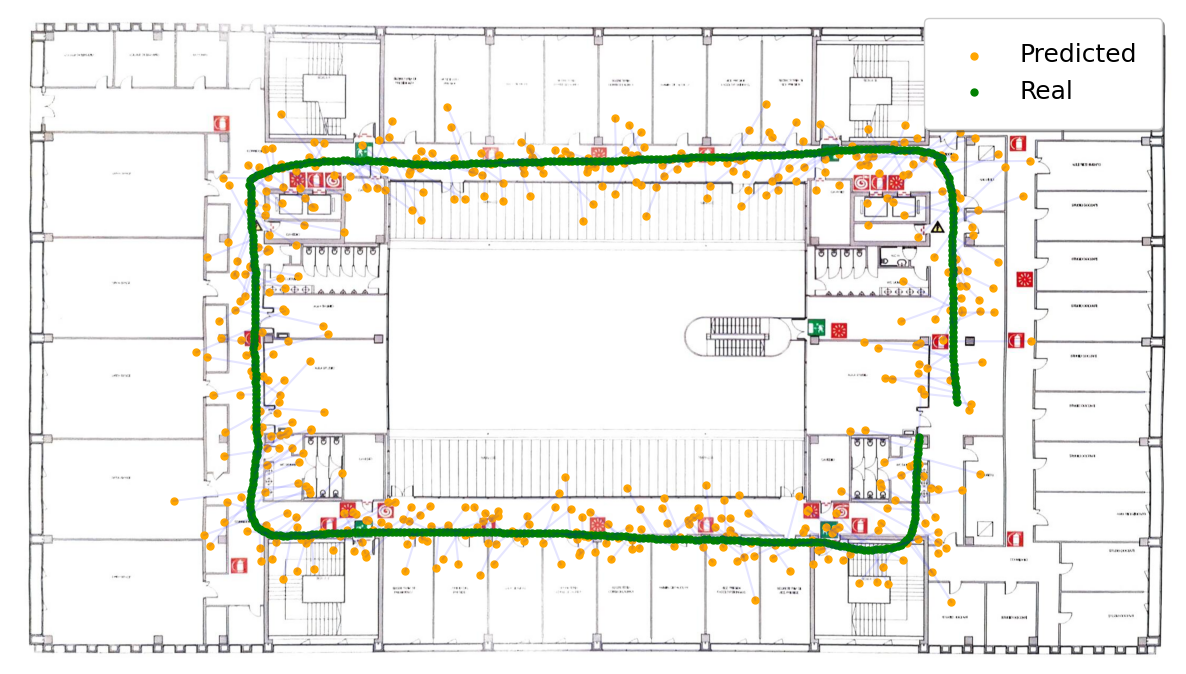
\includegraphics[width=0.9\textwidth]{../imgs/mapnet_map.png}
        \caption{MapNet predictions for our custom dataset. Error = $153cm$.}
    \end{figure}
\end{frame}
% Post-processing: new trajectory with new error
\begin{frame}{Detection of Non-Walkable Predictions}
    We developed post-processing algorithm to improve the model prediction: in case of a non-walkable spot, the output is corrected with the nearest \textbf{walkable} point according to the Euclidean distance criterion.
    \begin{figure}
        \centering
        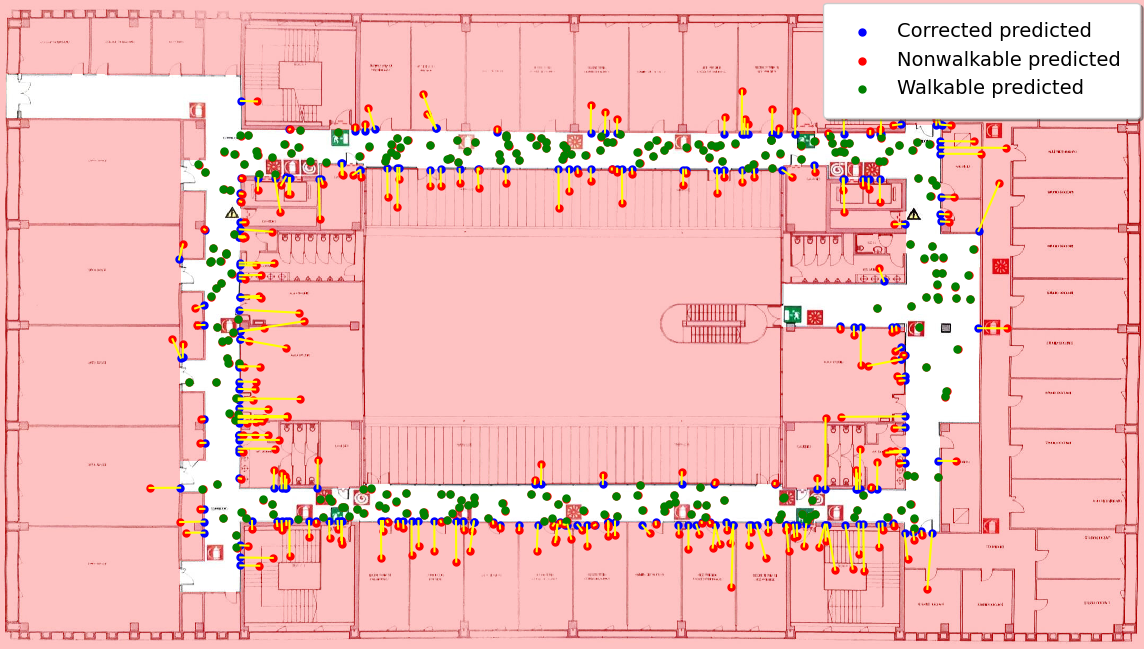
\includegraphics[width=0.7\textwidth]{../imgs/walkable_postprocess.png}
        \caption{Prediction map after the post-processing procedure. Error = $130cm$.}
    \end{figure}
\end{frame}
% Dashboard screen
\begin{frame}{Model Deployment with a Web-Server}
    \begin{figure}
        \centering
        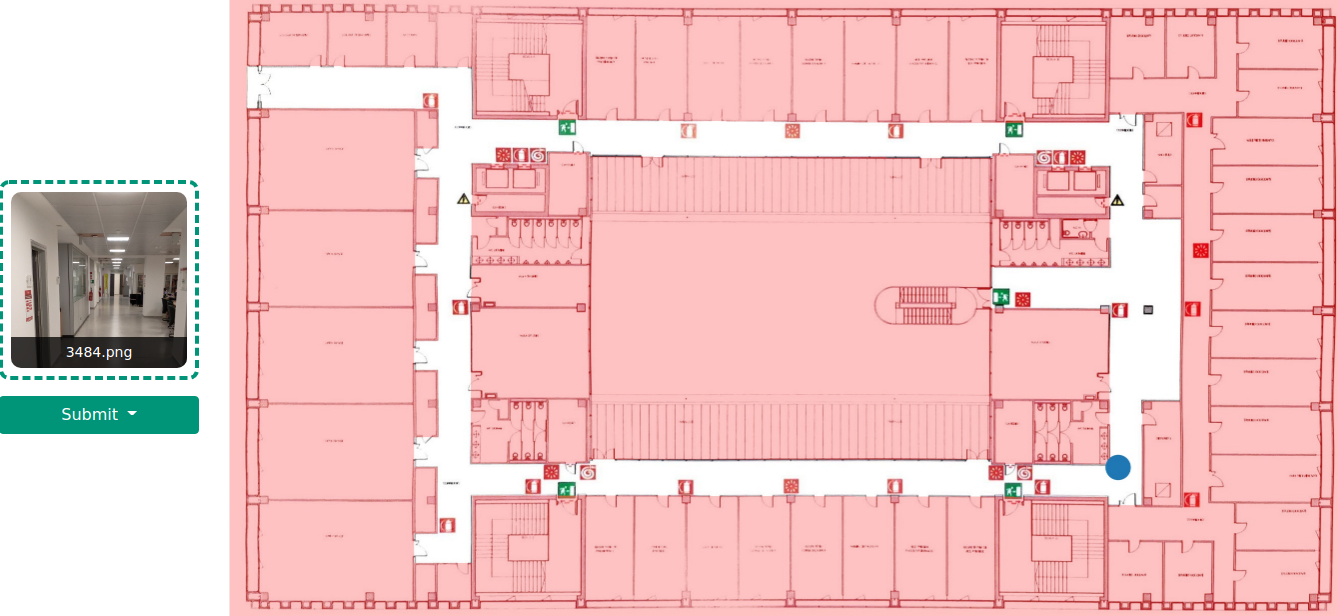
\includegraphics[width=0.9\textwidth]{../imgs/dashboard.png}
        \caption{FastAPI dashboard that serves the model.}
    \end{figure}
\end{frame}

\section{Conclusions}
\begin{frame}{Conclusions}
    To summarize, the final results presented in this work are:
    \begin{itemize}
        \item the exploration of multiple dataset generation techniques;
        \item the COLMAP reconstruction of Povo 1 second floor;
        \item the development of relative and absolute pose estimation models;
        \item the fine-tuning of absolute pose estimation models;
        \item the post-processing of the model outputs;
        \item the model deployment using a FastAPI web-server.
    \end{itemize}
\end{frame}

% \begin{frame}{Block examples}
%     \begin{block}{Observation 1}
%         Simmons Hall is composed of metal and concrete.
%     \end{block}
%     \begin{exampleblock}{Observation 2}
%         Simmons Hall is composed of metal and concrete.
%     \end{exampleblock}
%     \begin{textbfblock}{Conclusion}
%         Simmons Hall $\not=$ Simmons Dormitory.
%     \end{textbfblock}
% \end{frame}
\end{document}
